\documentclass[a4paper,12pt]{article}

\usepackage[T2A]{fontenc}			
\usepackage[utf8]{inputenc}			
\usepackage[english,russian]{babel}	

\usepackage[
bookmarks=true, colorlinks=true, unicode=true,
urlcolor=black,linkcolor=black, anchorcolor=black,
citecolor=black, menucolor=black, filecolor=black,
]{hyperref}

\usepackage{color}
\usepackage{caption}
\DeclareCaptionFont{white}{\color{black}}
\DeclareCaptionFormat{listing}{\colorbox{white}{\parbox{\textwidth}{#1#2#3}}}
\captionsetup[lstlisting]{format=listing,labelfont=white,textfont=white}

\usepackage{amsmath,amsfonts,amssymb,amsthm,mathtools} 
\usepackage{wasysym}

\usepackage{graphicx}
%\usepackage[cache=false]{minted}
\usepackage{cmap}
\usepackage{indentfirst}

\usepackage{listings} 
\usepackage{fancyvrb}

\usepackage{geometry}
\geometry{left=2cm}
\geometry{right=1.5cm}
\geometry{top=1cm}
\geometry{bottom=2cm}

\setlength{\parindent}{5ex}
\setlength{\parskip}{0.5em}

\usepackage{pgfplots}
\usetikzlibrary{datavisualization}
\usetikzlibrary{datavisualization.formats.functions}

\begin{document}
	\lstset{ %
		language=C,                 % выбор языка для подсветки (здесь это С)
		basicstyle=\small\sffamily, % размер и начертание шрифта для подсветки кода
		numbers=left,               % где поставить нумерацию строк (слева\справа)
		numberstyle=\tiny,           % размер шрифта для номеров строк
		stepnumber=1,                   % размер шага между двумя номерами строк
		numbersep=5pt,                % как далеко отстоят номера строк от подсвечиваемого кода
		backgroundcolor=\color{white}, % цвет фона подсветки - используем \usepackage{color}
		showspaces=false,            % показывать или нет пробелы специальными отступами
		showstringspaces=false,      % показывать или нет пробелы в строках
		showtabs=false,             % показывать или нет табуляцию в строках
		frame=single,              % рисовать рамку вокруг кода
		tabsize=2,                 % размер табуляции по умолчанию равен 2 пробелам
		captionpos=t,              % позиция заголовка вверху [t] или внизу [b] 
		breaklines=true,           % автоматически переносить строки (да\нет)
		breakatwhitespace=false, % переносить строки только если есть пробел
		escapeinside={\%*}{*)}   % если нужно добавить комментарии в коде
	}
	
	% Титульный лист
	\begin{figure}[h!]
		\begin{center}
			{
\includegraphics[scale = 0.4]{titul.jpg}}
			\label{titul}
		\end{center}
	\end{figure}
	
	\vspace*{15mm} 
	
	\huge
	\begin{center}
		Дисциплина: <<Функциональное и логическое программирование>>
	\end{center}
	\vspace*{15mm} 	
	
	\begin{center}
		Лабораторная работа №4
	\end{center}
	
	\vspace*{15mm} 	
	
	\large
	\begin{flushright}
		Студент: Левушкин И. К. \\
		Группа: ИУ7-62Б \\
		Преподаватели: Толпинская Н. Б., \\ Строганов Ю. В. \\
	\end{flushright}
	
	\vspace*{30mm}
	\begin{center}
		Москва, 2020 г.  
	\end{center}
	\thispagestyle{empty}
	
	
	\newpage
	
	\section*{6. Дана функция (defun mystery (x) (list (second x) (first x))).
Какие результаты вычисления следующих выражений?}
	
	\begin{table} [h!]
		\begin{center}
			\begin{tabular}{|l|l|}
				\hline
				{\bf  Выражение} &    {\bf Результат} \\
				\hline
				{(mystery (one two))} & error: undefined function ONE\\
				\hline
				{(mystery (last one two))} & error: variable ONE has no value\\
				\hline
				{(mystery free)} & error: variable FREE has no value\\
				\hline
				{(mystery one 'two))} & error: variable ONE has no value\\
				\hline
			\end{tabular}  
			\label{m1}
		\end{center}
	\end{table}

	\section*{7. Написать функцию, которая переводит температуру в системе Фаренгейта
температуру по Цельсию (defum f-to-c (temp)…).
}
	
	Формулы: 	c = 5/9*(f-320); 	f= 9/5*c+32.0.
	
	Ответ: \textit{(defun f-to-c (temp) (* (/ 5.0 9.0) (- temp 320)) )}
	
	
	Как бы назывался роман Р.Брэдбери "+451 по Фаренгейту" в системе по Цельсию?
	
	Ответ: \textit{72.77778}
	
	
	
	\section*{8. Что получится при вычисления каждого из выражений?}
	
	\begin{table} [h!]
		\begin{center}
			\begin{tabular}{|l|l|}
				\hline
				{\bf  Выражение} &    {\bf Результат} \\
				\hline
				{(list 'cons t NIL)} & (CONS T NIL)\\
				\hline
				{(eval (eval (list 'cons t NIL)))} & error: undefined function T\\
				\hline
				{(apply \#cons "(t NIL))} & error: bad syntax for complex number: \#CONS\\
				\hline
				 {(list 'eval NIL)} & (EVAL NIL)\\
				 \hline
				 {(eval (list 'cons t NIL))} & (T)\\
				 \hline
				 {(eval NIL)} & NIL\\
				 \hline
				 {(eval (list 'eval NIL))} & NIL\\
				 \hline
			\end{tabular}  
			\label{m2}
		\end{center}
	\end{table}
	
	\newpage]
	
	\section*{Написать функцию, вычисляющую катет по заданной гипотенузе и другому катету прямоугольного треугольника, и составить диаграмму ее вычисления.}
	
	Ответ: \textit{(defun func (gip kat) (sqrt (- (* gip gip) (* kat kat)) ) )}
	
	\newpage
	
	\section*{Написать функцию, вычисляющую площадь трапеции по ее основаниям и
высоте, и составить диаграмму ее вычисления.
}
	
	Ответ: \textit{(defun f (a b h) (* 0.5 (* h (+ a b))))}
	
	\newpage
	
	\section*{Ответы на вопросы}
	
	\subsection*{Как синтаксически представляется программа на Lisp? Как она хранится в памяти?}
	
	Программа и обрабатываемые ею данные представляются в Lisp одинаково:
	и то, и другое представляется списочной структурой. По этой причине программы могут обрабатывать и преобразовывать другие программы и свою собственную.
	
	\subsection*{Как трактуются элементы списка?}
	
	Перый элемент трактуется как имя функции, остальные элементы - как аргументы. Если стоит блокировка вычисления (функция QUOTE, или в сокращенном виде '), то первый элемент также трактуется как аргумент.
	
	\subsection*{Порядок реализации программы}
	
	Программа работает в цикле:
	\begin{itemize}
		\item Ожидание ввода S-выражения
		\item Передача введенного S-выражения функции EVAL
		\item Вывод полученного результата
	\end{itemize}
	 \newpage
	\subsection*{Работа функции EVAL}
	
	\begin{figure}[h!]
		\begin{center}
			{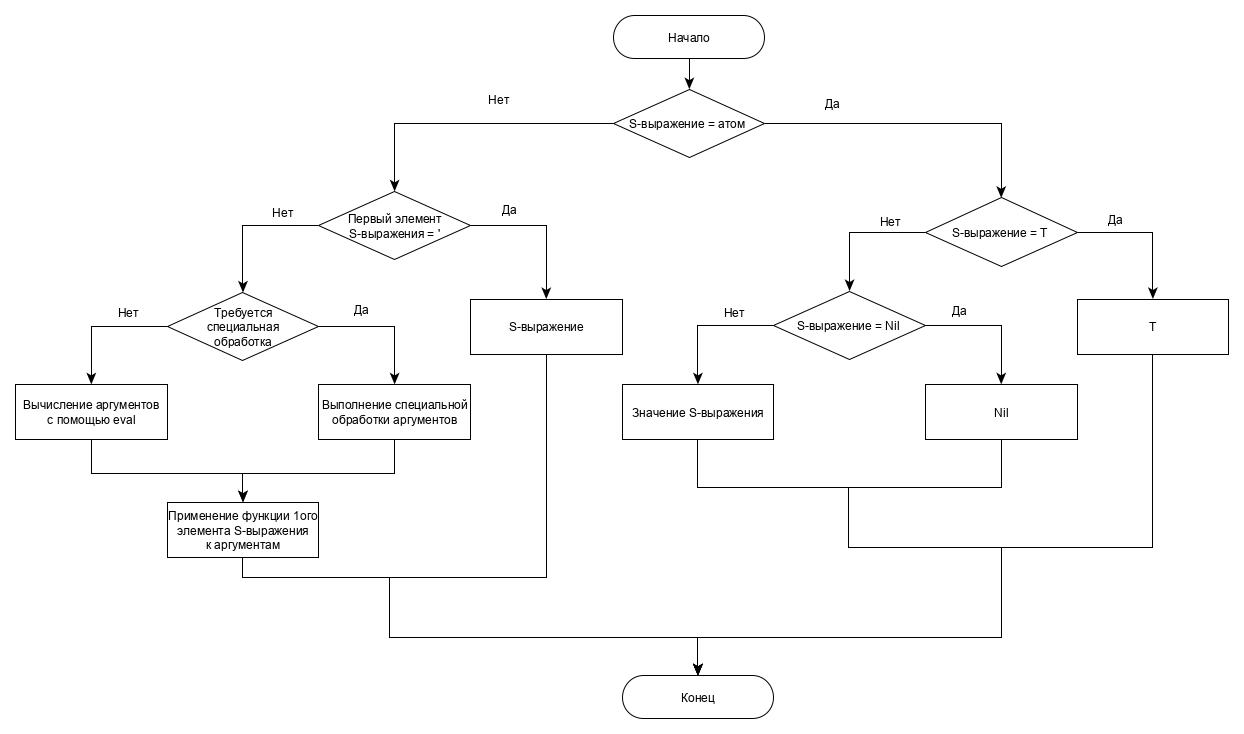
\includegraphics[scale = 0.4]{eval.jpg}}
			\label{eval}
		\end{center}
	\end{figure}

\end{document}